\begin{figure}[H]
  \centering

  \begin{subfigure}[b]{0.2\textwidth}
    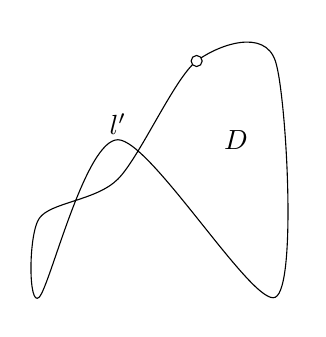
\begin{tikzpicture}
      
      \draw plot [smooth cycle] coordinates {
        (0, 0) (0, 1) (1, 1.5) (2, 3) (3, 3) (3, 0) (1, 2)
      };
      \draw[draw = black, fill = white] (2, 3) circle (2pt);
      \draw node at (2.5, 2) {\(D\)};
      \draw node at (1, 2.2) {\(l'\)};

    \end{tikzpicture}

  \caption{\(l'\) - не простая граница}\label{fig:area-prop-4-a}
  \end{subfigure}
  \qquad
  \begin{subfigure}[b]{0.2\textwidth}
    \begin{tikzpicture}

      \draw plot [smooth cycle] coordinates {
        (0, 0) (0, 1) (1, 1.5) (2, 3) (3, 3) (3, 0)
      };
      \draw node at (2, 1) {\(D\)};
      \draw node at (1, 2) {\(l\)};

    \end{tikzpicture}
    \caption{\(l\) - простая граница}\label{fig:area-prop-4-b}
  \end{subfigure}
\end{figure}